\chapter{Testing and Results}
\label{ch:results}

% This section should write itself. Since you have a goal, the results section must document that you have reached this goal (or verified your hypothesis).

%-------------------------
\section{Experiment Setup}

\paragraph{Implementation} We have implemented a full framework for robust web extraction in Java. The logic is packaged as a \emph{Java Archive} component for easy use in other projects. We have used this component to carry out an experiment, which is described below. For details on the implementation and the dataset please refer to the project homepage at \url{https://bitbucket.org/mantiniss/thesis-wrapper}.

\paragraph{Test data set} To test the performance of our algorithm, we used snapshots of web pages from the \emph{Internet Archive} (\url{archive.org}). In particular, we focused on two websites: an e-commerce website \url{amazon.com} for extracting book listings and a movie database \url{imdb.com} for extracting movie titles.

For each of the websites, we chose a random HTML document with a list of data records, e.g. a list of books or a list of movies. For \url{amazon.com} we picked \emph{Most Popular TV Series, Feature Films, TV Movies} page and for \url{imdb.com} we chose \emph{Books: Last 30 days} page. We collected a set of 10 snapshots of the each page over extensive period. The details of both datasets are provided in Figure~\ref{tbl:dataset}.

\begin{figure}[h]
	\centering
    \begin{tabularx}{\textwidth}{ | X | c | c | }
		\hline
		\textbf{Website} & \url{imdb.com} & \url{amazon.com} \\
		\hline
		\textbf{Number of page snapshots} & 10 & 10 \\
		\hline
		\textbf{Earliest crawl time} & 20 Oct, 2014 & 25 Feb, 2014 \\
		\hline
		\textbf{Latest crawl time} & 30 Dec, 2014 & 26 Aug, 2014 \\
		\hline
		\textbf{Number of data records per page} & 100 & 12 \\
		\hline
		\textbf{Average tree size} & 5521 & 2223 \\
		\hline
    \end{tabularx}
	\caption{Dataset details (source: \emph{Internet Archive}).}
	\label{tbl:dataset}
\end{figure}

\paragraph{Distinguished nodes} We marked a single distinguished node on each HTML document by manually writing XPath queries: \texttt{//*[@id="result\_0"]/div[4]/h3/a} and \texttt{//*[@id="main"]/table/tbody/tr[2]/td[3]/a}. After the wrapper extracted data record attributes, we manually checked the number of results and the correctness of the data returned. We tested the correctness by seeing, if the result contains the right attribute value from a data records. The process was completely manual, but considering the small dataset we decided to keep it that way.

Thinking about a larger data set, the process of results verification could be automated following a method by Parameswaran et al. \cite{DBLP:journals/pvldb/ParameswaranDGR11}. In his experiment, the author chose to extract easily verifiable piece of information, e.g. vote count which matches a pattern "\{n\} votes". Thus the process could be automated by matching extracted results against this pattern. Due to limited time, we chose not to automate certain parts of the experiment.

\paragraph{Probabilistic change model} Learning probabilities of HTML element transformations, i.e. change model, is out of the scope of this project. Thus, we set the probabilities for insert, delete, and substitute operations to the same value. By using the same change model for all tests, we avoided bias and focused on core wrapping comparison. Although, learning and improving the change model as we wrap more web pages, would definitely be an interesting direction to explore.


%---------------------------
\section{Evaluation Metrics}

The test takes an initial version of an HTML document, a distinguished node, and a transformed HTML document as an input. As an output, the test returns a list of extracted data record attribute values. For each execution we manually check the count and the correctness of the returned results.

\paragraph{Accuracy} As a primary measure of success, we track the number of data records returned correctly. That is, if the transformed HTML document contains 20 data records, and our wrapper correctly locates and extracts information from 18 items, we measure our accuracy as $18 / 20 = 90\%$. The higher the accuracy, the better our algorithm performs.

\paragraph{Skip sizes} We measure how well our wrapper performs with relation to the time between initial and transformed HTML document snapshots. We use \emph{skip size} as a relative measure of time between document versions. A pair of snapshots have a skip size of $k$, if the second snapshot was taken roughly $k$ weeks after the first one. The larger the skip size, the higher the probability that the page has evolved. In our experiment, we vary skip sizes ($k = 1, 2, 3$) for each data set.

\paragraph{Execution time} We also measure the time taken to extract multiple data record attributes. Since reasonable execution time is one of the goals for the wrapper, this measure is important. We perform our test on \emph{Intel Core i5-2410M} processor running at 2.30 GHz on 4 cores.


%---------------------------
\section{Experiment Results}

\paragraph{Input and output} In the experiment, we ran the wrapper for three skip sizes ($k = 1, 2, 3$) and plotted the results in a Figure~\ref{fig:accuracy}. The vertical axis represents the percentage of time the wrapper succeeded. Each bar displays an average accuracy per data set. For example, for a skip size $k=1$ in \url{amazon.com} we executed the algorithm 9 times with the following params: $(w_1,w_2,d(w_1))$, $(w_2,w_3,d(w_2))$, etc. We counted how many data records were extracted correctly and divided that number by a total data record count. The resulting accuracy measure was averaged over 9 runs.

\paragraph{Execution time} The average wrapping time for \url{amazon.com} data set was around $0.8$ seconds, and for \url{imdb.com} -- around $1.7$ seconds.

\begin{figure}[h]
	\centering
	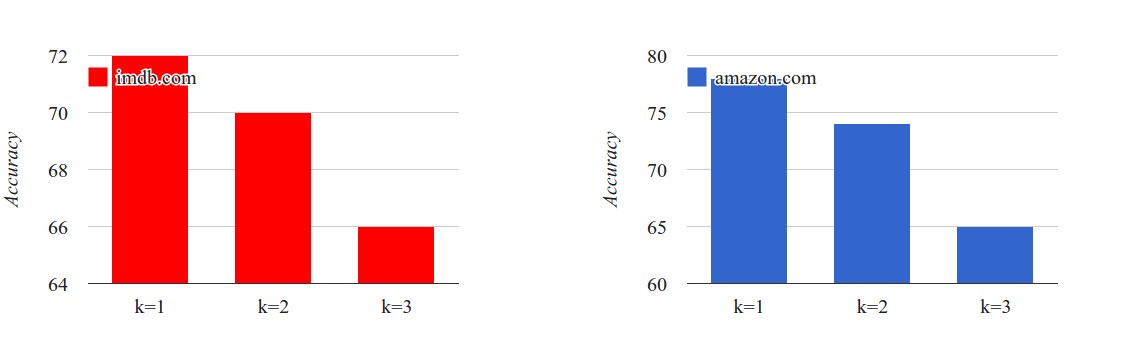
\includegraphics[width=1.0\textwidth]{figures/accuracy}
	\caption{Experiment results from (a) \url{imdb.com} and (b) \url{amazon.com} websites.}
	\label{fig:accuracy}
\end{figure}

\paragraph{Accuracy} Figures~\ref{fig:accuracy}(a) and \ref{fig:accuracy}(b) contain the results for \url{imdb.com} and \url{amazon.com} respectively. As can be seen from the charts, the average accuracy was similar for both websites, i.e. around $70\%$. 


%-------------------
\section{Discussion}

Overall, the experiment proves that the idea of using probabilistic web wrapper to extract from multiple records is viable.

When compared to $85\%-95\%$ accuracy of a probabilistic page-level wrapper by Parameswaran et al. \cite{DBLP:journals/pvldb/ParameswaranDGR11}, our wrapper implementation performed worse. Yet, it is important to note that the data set in our experiment was different from the one Parameswaran used. In addition, our wrapper had to extract multiple records versus a single one by Parameswaran.

Another observation is that for both websites there was a drop in accuracy as the skip size increased. That is an expected outcome as the more pages evolve, the larger the differences become.

In all cases the data records were correctly identified. It would be interesting to test the data record locator with non-contigouos data regions or records that are not wrapped in a table. Due to the tight schedule, these tests were not conducted as part of the experiment.


% vim:wrap linebreak nolist:
